\begin{center}
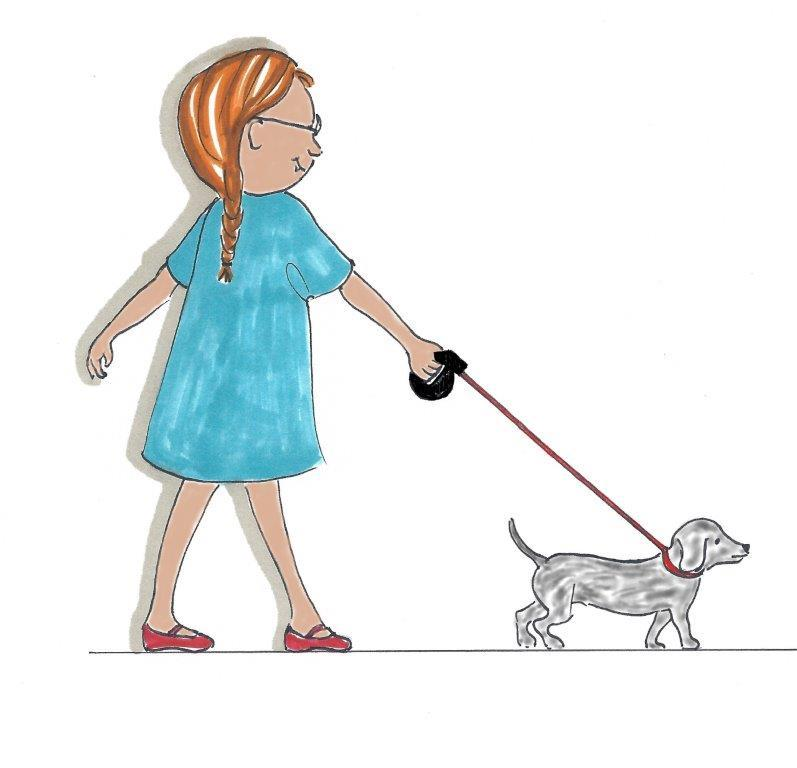
\includegraphics[width=0.6\textwidth]{content/3/chapter5/images/3.png}\\
Cippi walks the dog
\end{center}

A std::span stands for an object that refers to a contiguous sequence of objects. A std::span, sometimes also called a view, is never an owner. This contiguous sequence of objects can be a plain C-array, a pointer with a size, a std::array, a std::vector, or a std::string.

A std::span can have a static extent or a dynamic extent. By default, std::span has a dynamic extent:

\noindent
Definition of std::span
\begin{lstlisting}[style=styleCXX]
template <typename T, std::size_t Extent = std::dynamic_extent>
class span;
\end{lstlisting}

\subsubsubsection{5.2.1\hspace{0.2cm} Static versus Dynamic Extent}

When a std::span has a static extent, its size is known at compile time and part of the type: std::span<T, size>. Consequently, its implementation needs only a pointer to the first element of the contiguous sequence of objects.

Implementing a std::span with a dynamic extent consists of a pointer to the first element and the size of the contiguous sequence of objects. The size is not part of the type: std::span<T>.

The next example staticDynamicExtentSpan.cpp emphasizes the differences between both kinds of views.

\noindent
std::spans with static and dynamic extent
\begin{lstlisting}[style=styleCXX]
// staticDynamicExtentSpan.cpp

#include <iostream>
 #include <span>
 #include <vector>

void printMe(std::span<int> container) {
	
	std::cout << "container.size(): " << container.size() << '\n';
	for (auto e : container) std::cout << e << ' ';
	std::cout << "\n\n";
}

int main() {

	std::cout << '\n';
	
	std::vector myVec1{1, 2, 3, 4, 5};
	std::vector myVec2{6, 7, 8, 9};
	
	std::span<int> dynamicSpan(myVec1);
	std::span<int, 4> staticSpan(myVec2);
	
	printMe(dynamicSpan);
	printMe(staticSpan); // implicitly converted into a dynamic span
	
	// staticSpan = dynamicSpan; ERROR
	dynamicSpan = staticSpan;
	
	printMe(staticSpan);
	
	std::cout << '\n';

}
\end{lstlisting}

dynamicSpan (line 21) has a dynamic extent, while staticSpan (line 22) has a static extent. Both std::spans return their size in the printMe function (line 9). A std::span with dynamic extent can be assigned to a std::span with static extent, but not the other way around. Line 27 would cause an error, but lines 7, 25 and 28 are valid.

\begin{center}
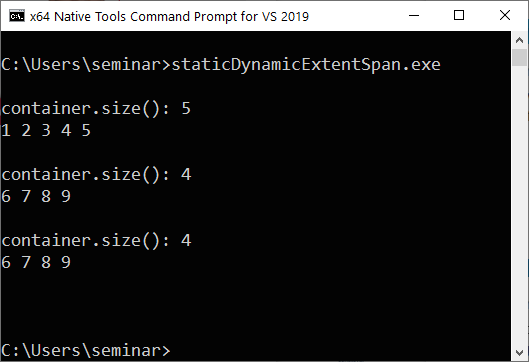
\includegraphics[width=0.6\textwidth]{content/3/chapter5/images/4.png}\\
std::spans with static and dynamic extent
\end{center}

One important reason for having a std::span<T> is that a plain C-array \href{https://en.cppreference.com/w/cpp/types/decay}{decays} to a pointer if passed to a function; therefore, the size is lost. This decay is a typical reason for errors in C/C++.

\subsubsubsection{5.2.2\hspace{0.2cm} Automatically Deduces the Size of a Contiguous Sequence of Objects}

In contrast to a C-array, std::span<T> automatically deduces the size of contiguous sequences of objects.

\noindent
A std::span automatically deduces the size of its referenced sequence of object
\begin{lstlisting}[style=styleCXX]
// printSpan.cpp

#include <iostream>
#include <vector>
#include <array>
#include <span>

void printMe(std::span<int> container) {

	std::cout << "container.size(): " << container.size() << '\n';
	for (auto e : container) std::cout << e << ' ';
	std::cout << "\n\n";
	
}

int main() {

	std::cout << '\n';
	
	int arr[]{1, 2, 3, 4};
	printMe(arr);
	
	std::vector vec{1, 2, 3, 4, 5};
	printMe(vec);
	
	std::array arr2{1, 2, 3, 4, 5, 6};
	printMe(arr2);

}
\end{lstlisting}

The C-array (line 19), std::vector (line 22), and the std::array (line 25) contain int values. Consequently, std::span also holds int values. There is something more interesting in this simple example. For each container, std::span can deduce its size (line 10).

\begin{center}
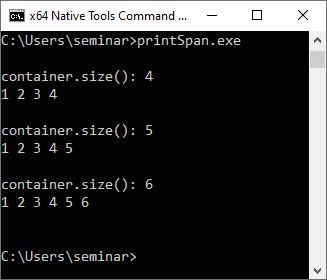
\includegraphics[width=0.6\textwidth]{content/3/chapter5/images/5.png}\\
Automatic size deduction of a std::span
\end{center}

There are more ways to create a std::span.


\subsubsubsection{5.2.3\hspace{0.2cm} Create a std::span from a Pointer and a Size}

You can create a std::span from a pointer and a size.

\noindent
Create a std::span
\begin{lstlisting}[style=styleCXX]
// createSpan.cpp

#include <algorithm>
#include <iostream>
#include <span>
#include <vector>

int main() {
	
	std::cout << '\n';
	std::cout << std::boolalpha;
	
	std::vector myVec{1, 2, 3, 4, 5};
	
	std::span mySpan1{myVec};
	std::span mySpan2{myVec.data(), myVec.size()};
	
	bool spansEqual = std::equal(mySpan1.begin(), mySpan1.end(),
	                             mySpan2.begin(), mySpan2.end());
	
	std::cout << "mySpan1 == mySpan2: " << spansEqual << '\n';
	
	std::cout << '\n';

}
\end{lstlisting}

As you may expect, mySpan1, created from the std::vector (line 15), and mySpan2, created from a pointer and a size (line 16), are equal (line 21).

\begin{center}
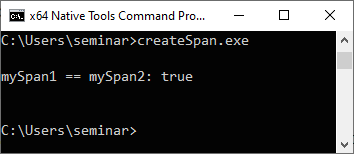
\includegraphics[width=0.6\textwidth]{content/3/chapter5/images/6.png}\\
Create a std::span from a pointer and a size
\end{center}

\begin{tcolorbox}[colback=red!5!white,colframe=red!75!black,title={A std::span is neither a std::string\_view nor a view}]
You may remember that a std::span is sometimes called a view. Don’t confuse a std::span with a view from the ranges library or a \href{https://www.modernescpp.com/index.php/c-17-what-s-new-in-the-library}{std::string\_view}.

A view from the ranges library is something that you can apply on a range and performs some operation. A view does not own data, and its time for each copy, move, and assignment is constant. A std::span and a std::string\_view are non-owning views and can deal with strings.

The main difference between a std::span and a std::string\_view is that a std::span can modify its referenced objects.
\end{tcolorbox}
	
\subsubsubsection{5.2.4\hspace{0.2cm} Modifying the Referenced Objects}

You can modify an entire span or only a subspan. When you modify a span, you modify the referenced objects.

The following program shows how a subspan can be used to modify the referenced objects from a std::vector.

\noindent
Modify the objects referenced by a std::span
\begin{lstlisting}[style=styleCXX]
// spanTransform.cpp

#include <algorithm>
 #include <iostream>
 #include <vector>
 #include <span>

void printMe(std::span<int> container) {
	
	 std::cout << "container.size(): " << container.size() << '\n';
	 for (auto e : container) std::cout << e << ' ';
	 std::cout << "\n\n";
}

int main() {

	std::cout << '\n';
	
	std::vector vec{1, 2, 3, 4, 5, 6, 7, 8, 9, 10};
	printMe(vec);
	
	std::span span1(vec);
	std::span span2{span1.subspan(1, span1.size() - 2)};
	
	
	std::transform(span2.begin(), span2.end(),
	               span2.begin(),
	               [](int i){ return i * i; });
	
	
	printMe(vec);
	printMe(span1);

}
\end{lstlisting}

span1 references the std::vector vec (line 22). In contrast, span2 references only the elements of the underlying vec excluding the first and the last element (line 23). Consequently, the mapping of each element to its square (line 26) only addresses these elements.

\begin{center}
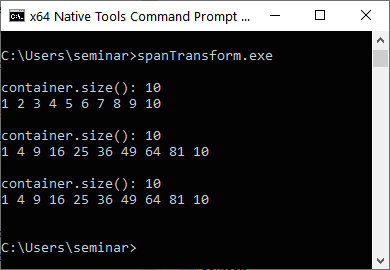
\includegraphics[width=0.6\textwidth]{content/3/chapter5/images/7.png}\\
Modify the objects referend by a std::span
\end{center}

There are various convenience functions to address the elements of the std::span.

\subsubsubsection{5.2.5\hspace{0.2cm} Addressing std::span Elements}

The following table presents the functions to refer to the elements of a std::span.

\begin{center}
Interface of a std::span spse
\end{center}

\begin{table}[H]
\centering
\begin{tabular}{ll}
Function         & Description                                         \\ \hline
sp.front()       & Access the first element.                           \\
sp.back()        & Access the last element.                            \\
sp{[}i{]}        & Access the i-th element.                            \\
sp.data()        & Returns a pointer to the beginning of the sequence. \\
sp.size()        & Returns the number of elements of the sequence.     \\
sp.size\_bytes() & Returns the size of the sequence in bytes.          \\
sp.empty()       & Returns true if the sequence is empty.              \\
\begin{tabular}[c]{@{}l@{}}sp.first\textless{}count\textgreater{}()\\ sp.frist(count)\end{tabular} &
Returns a subspan consisting of the first count elements of the sequence. \\
\begin{tabular}[c]{@{}l@{}}sp.last\textless{}count\textgreater{}()\\ sp.last(count)\end{tabular} &
Returns a subspan consisting of the last count elements of the sequence. \\
\begin{tabular}[c]{@{}l@{}}sp.subspan\textless{}first, count\textgreater{}()\\ sp.subspan(first, count)\end{tabular} &
Returns a subspan consisting of count elements starting at first.
\end{tabular}
\end{table}

The program subspan.cpp shows the usage of the member function subspan.

\noindent
Use of the member function subspan
\begin{lstlisting}[style=styleCXX]
// subspan.cpp

#include <iostream>
#include <numeric>
#include <span>
#include <vector>

int main() {

	std::cout << '\n';
	
	std::vector<int> myVec(20);
	std::iota(myVec.begin(), myVec.end(), 0);
	for (auto v: myVec) std::cout << v << " ";
	
	std::cout << "\n\n";
	
	std::span<int> mySpan(myVec);
	auto length = mySpan.size();
	
	std::size_t count = 5;
	for (std::size_t first = 0; first <= (length - count); first += count ) {
		for (auto ele: mySpan.subspan(first, count)) std::cout << ele << " ";
		std::cout << '\n';
	}

}
\end{lstlisting}

Line 13 fills the vector with all numbers from 0 to 19 (line 13) using the algorithm \href{https://en.cppreference.com/w/cpp/algorithm/iota}{std::iota}. This vector is further used to initialize a std::span (line 18). Finally, the for loop (line 22) uses the function subspan to create all subspans starting at first and having count elements until mySpan is consumed.

\begin{center}
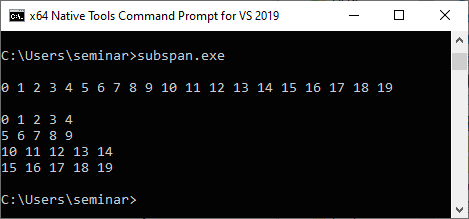
\includegraphics[width=0.6\textwidth]{content/3/chapter5/images/8.png}\\
Use of the member function subspan
\end{center}

Kilian Henneberger reminded me of a special use case of std::span. A constant range of modifiable elements.

\subsubsubsection{5.2.6\hspace{0.2cm} A Constant Range of Modifiable Elements}

For simplicity, I name a std::vector and a std::span a range. A std::vector, like a std::string models a modifiable range of modifiable elements: std::vector<T>. When you declare this std::vector as const, the range models a constant range of constant objects: const std::vector<T>. You cannot model a constant range of modifiable elements. Here comes std::span into play. A std::span models a constant range of modifiable objects: std::span<T>. The following table emphasizes the variations of (constant/modifiable) ranges and (constant/modifiable) elements.

\begin{center}
(Constant/modifiable) ranges of (constant/modifiable) elements
\end{center}

\begin{table}[H]
\centering
\begin{tabular}{lll}
&
\textbf{Modifiable Elements} &
\textbf{Constant Elements} \\
\textbf{Modifiable Ranges} &
std::vector\textless{}T\textgreater{} &
\\
\textbf{Constant Ranges} &
std::span\textless{}T\textgreater{} &
\begin{tabular}[c]{@{}l@{}}const std::vector\textless{}T\textgreater\\ std::span\textless{}const T\textgreater{}\end{tabular}
\end{tabular}
\end{table}

The program constRangeModifiableElements.cpp exemplifies each combination.

\noindent
(Constant/modifiable) ranges of (constant/modifiable) elements
\begin{lstlisting}[style=styleCXX]
// constRangeModifiableElements.cpp

#include <iostream>
#include <span>
#include <vector>

void printMe(std::span<int> container) {

	std::cout << "container.size(): " << container.size() << '\n';
	for (auto e : container) std::cout << e << ' ';
	std::cout << "\n\n";
}

int main() {

	std::cout << '\n';
	
	std::vector<int> origVec{1, 2, 2, 4, 5};
	
	// Modifiable range of modifiable elements
	std::vector<int> dynamVec = origVec;
	dynamVec[2] = 3;
	dynamVec.push_back(6);
	printMe(dynamVec);
	
	// Constant range of constant elements
	const std::vector<int> constVec = origVec;
	// constVec[2] = 3; ERROR
	// constVec.push_back(6); ERROR
	std::span<const int> constSpan(origVec);
	// constSpan[2] = 3; ERROR
	
	// Constant range of modifiable elements
	std::span<int> dynamSpan{origVec};
	dynamSpan[2] = 3;
	printMe(dynamSpan);
	
	std::cout << '\n';

}
\end{lstlisting}

The vector dynamVec (line 21) is a modifiable range of modifiable elements. This observation does not hold for the vector constVec (line 27). Neither can constVec change an element nor its size. constSpan (line 30) behaves accordingly. dynamSpan models the unique use case of a constant range of modifiable elements.

\begin{center}
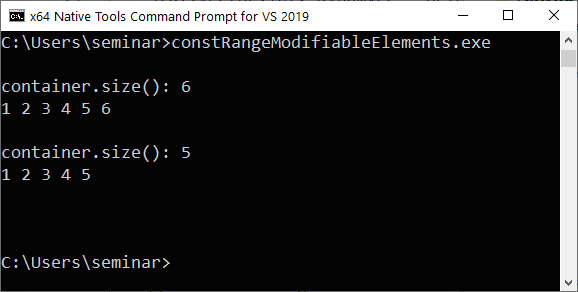
\includegraphics[width=0.6\textwidth]{content/3/chapter5/images/9.png}\\
(Constant/modifiable) ranges of (constant/modifiable) elements
\end{center}

\begin{tcolorbox}[colback=mygreen!5!white,colframe=mygreen!75!black,title={Distilled Information}]

\begin{itemize}
\item 
A std::span is an object that refers to a contiguous sequence of objects. A std::span, also known as view, is never an owner and, therefore, does not allocate memory. The contiguous sequence of objects can be a plain C-array, a pointer with a size, a std::array, a std::vector, or a std::string.

\item 
In contrast to a C-array, a std::span automatically deduces the size of its referenced sequence of objects.

\item 
When a std::span modifies its elements, the reference objects are also modified.
\end{itemize}

\end{tcolorbox}


\newpage








